\begin{center}\large\textbf{Readings: Chapter 5 (for 5.8-5.9 read if interested)}\\
\normalsize \end{center}
\large ~\hrulefill
~\\
\normalsize Recall our overall idea:
\begin{center}
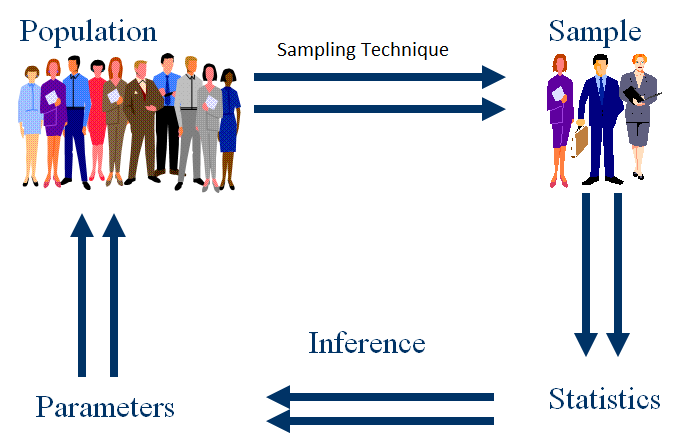
\includegraphics[scale=0.55]{paradigm}
\end{center}

~\\~\\~\\~\\~\\
Inference - refers to making mathematical claims about a parameter using sample data.\\~\\
Two main methods for inference:\\
\begin{enumerate}
\item \underbar{~~~~~~~~~~~~~~~~~~~~~~~~~~~~~~~~~~~~~~~~~~~~~~~~~~~} - Range of values we think contains the parameter.\\
\item \underbar{~~~~~~~~~~~~~~~~~~~~~~~~~~~~~~~~~~~~~~~~~~~~~~~~~~~} - Test of whether a specific parameter value is plausible.  
\end{enumerate}

\newpage

Putting it all together: Engineers at Ford are attempting to improve the overall gas mileage of next year's model of one of their cars.  From extensive testing on the previous year's model they know the gas mileage can be well modeled by a normal distribution with true mean gas mileage of 26.9 mpg and true standard deviation of 2.3 mpg.\\
To investigate if this year's model has improved the average gas mileage, data is collected on 16 automobiles.   The average gas mileage of the sample is 28.25 mpg.
\begin{itemize}
\item Population - \\
\item Parameter of Interest -\\~\\
\item Random Variables used to answer questions of interest - \\~\\~\\~\\~\\~\\
\begin{flushleft}
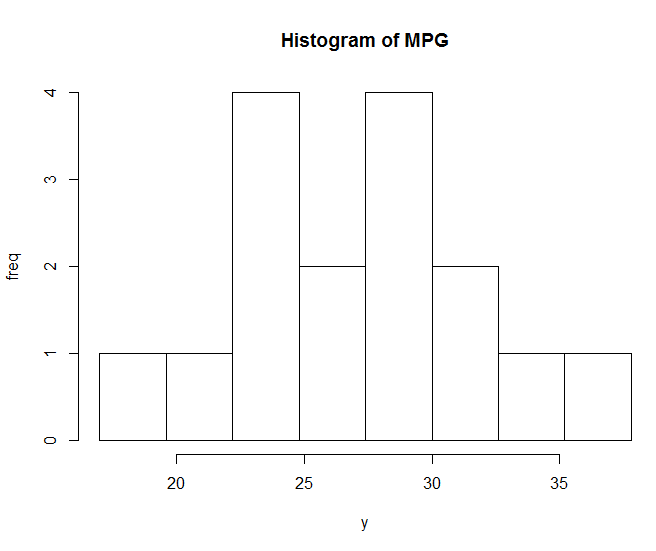
\includegraphics[scale=0.5]{mpg}
\end{flushleft}~\\~\\~\\
\item Sample - \\
\item Statistic(s) - \\

\newpage

\item Inference using a `Hypothesis Test' -

\newpage

\item Inference using a `Confidence Interval' - 
\end{itemize}

\newpage


\Large 5.2 - Confidence Intervals \\
\normalsize

Confidence Intervals are better than point estimates, such as $\bar{y}$, as they \underbar{~~~~~~~~~~~~~~~~~~~~~~~~~~~~~~~~~~~~~~~~~~~~~~~~}\\~\\~\\~\\~\\~\\~\\

Intervals that are created have a \underbar{~~~~~~~~~~~~~~~~~~~~~~~~~~~~~~~~~~~~~~~~~~~~~~~~~~~~~~~~~~~~~~~~~~~~~~~~~~~~~~~~~~~~~} = the probability \textbf{the procedure used} creates an interval that contains the parameter.\\~\\

$\alpha$ = \underbar{~~~~~~~~~~~~~~~~~~~~~~~~~~~~~~~~~~~~~~~~~~~~~~~~~~~~~~~~~~~~~~~~~~~~~~~~~~~~~~~~} - usually 0.01, 0.05, or 0.1.\\~\\

An \textbf{observed interval}, such as the one in the example above, is interpreted in the following manner:\\~\\
We say...\\~\\~\\~\\~\\~\\
For a confidence level of $(1-\alpha)$, the general interpretation of an observed CI is...\\~\\~\\~\\~\\~\\
What we mean by `confident' for our example above is...\\~\\~\\~\\~\\~\\~\\~\\
For a general $(1-\alpha)$100\% CI, confidence is interpreted as...\\~\\~\\~\\~\\~\\~\\~\\

Note that the interval is random and the parameter is fixed!\\
\begin{verbatim}
http://bcs.whfreeman.com/ips4e/cat_010/applets/confidenceinterval.html
\end{verbatim}

\newpage

\huge Confidence Interval for $\mu_Y$, the population mean \normalsize\\~\\
For a \textbf{random sample} of size $n$, where the population standard deviation, $\sigma_Y$, is known, a $(1-\alpha)100$\% CI for $\mu_Y$ is given by \\~\\~\\~\\~\\~\\
The interval is valid if \textbf{either}\begin{enumerate}
\item ~\\~\\
\item ~\\
\end{enumerate}

Common z values used:\\~\\~\\~\\~\\~\\~\\

Ex: The length of music videos is of interest to advertisers.  Assume we know the standard deviation of the length of music videos is 18 seconds (a dubious assumption we will learn to deal with later). In a random sample of 44 music videos, the average length was found to be 186 seconds. Find a 90\% confidence interval for the mean length of all music videos. What does confidence mean here?

\newpage
(Book examples 5.1 pg 228, 5.2 pg 229 for more practice.)\\~\\
Factors that affect the width of confidence intervals:
\begin{enumerate}
\item Natural Variability -\\~\\
\item Level of Confidence desired -\\~\\
\item Sample size $n$\\~\\~\\
\end{enumerate}

\Large 5.3 - Required sample size to have an interval of a given width: \normalsize \\~\\~\\~\\~\\~\\~\\~\\~\\~\\~\\~\\~\\~\\~\\~\\

Ex: Suppose that birth weights for boys are normally distributed.  We want to estimate the population mean $\mu$, the overall average birthweight for boys.  Assuming that the population standard deviation, $\sigma$, is known to be 12 oz (based on past data), what minimum sample size is required if the width of a 90\% CI is to be at most 6 ounces?\\~\\~\\~\\~\\~\\~\\~\\~\\~\\~\\~\\~\\

(Book examples 5.3/5.4 on page 231/232 for more practice.) 

\newpage

\Large 5.4/5.6 - Hypothesis Testing for $\mu_Y$. \normalsize\\
\begin{itemize}
\item Hypothesis testing and confidence interval estimation are related methods and are often both used to analyze the same situation.
\item CI is a numerical answer to the question, `What is the population value?'
\item Hypothesis test is used to answer questions about particular values for a parameter.
\end{itemize}

Goal of hypothesis testing: \\~\\~\\~\\~\\

\large Step 1/2 - Determine Null and Alternative Hypotheses\normalsize\\~\\~\\

\underbar{~~~~~~~~~~~~~~~~~~~~~~~~~~~~~~~~~~} - a statement or claim regarding parameter(s)\\~\\~\\
\underbar{~~~~~~~~~~~~~~~~~~~~~~~~~~~~~~~~~~~~~~~~~~~~~~~~~~~~~~~~~~~~~~~~~~~~~~~~~~~~} - Statement about parameter `no effect' or `no difference,' the default belief or status quo.\\~\\~\\
\underbar{~~~~~~~~~~~~~~~~~~~~~~~~~~~~~~~~~~~~~~~~~~~~~~~~~~~~~~~~~~~~~~~~~~~~~~~~~~~~} - Statement we hope to prove or give evidence for.\\~\\

One-sided vs Two-Sided Hypotheses:\\~\\~\\~\\~\\~\\~\\

For the following examples, define the parameter of interest and determine the null and alternative hypotheses:
\begin{enumerate}
\item A certain type of light bulb is advertised as having an average lifetime of 750 hours. A potential customer likes the price and wants to purchase a large amount of them if it can be shown the average lifetime is higher than advertised. A random sample of 20 bulbs was selected and the lifetime of each bulb was determined. The mean was 766.4 hours.  It is known that the lifetime of the light bulbs is normally distributed and the true standard deviation is 30.5 hours.

\newpage

\item The average age of a person on facebook last year was 19.34 years.  The standard deviation of the age of facebook users is 8.2 years.  Suppose an advertising agency is interested in seeing if the average age is different this year. He randomly selects 150 profiles and finds that the sample mean is 18.99 years old.\\~\\~\\~\\~\\~\\
\end{enumerate}

There are two possible conclusions from a hypothesis test: 
\begin{itemize}
\item ~
\begin{itemize}
\item Observed value is `significantly different' than hypothesized value (i.e. observed value is unlikely to have occurred simply due to random chance if the hypothesized value were true)
\end{itemize}	
\item ~\\
\end{itemize}	

We never `accept' $H_0$ as the book states. We believe the null hypothesis  until we see significant evidence to the contrary.  Thus, we either reject the null or we fail to reject (not enough evidence to the contrary).  This does not imply that $H_0$ is true, just that we can't say it isn't true.
\begin{itemize}
\item The data collected will not `prove $H_0$', but it may lead us to believe that it is pretty unlikely that $H_0$ is true.\\
\end{itemize}

Two types of errors we could make:\\
\begin{itemize}
\item \underbar{~~~~~~~~~~~~~~~~~~~~~~~~~~~~~~~~~~~~~~~~~~} - Reject $H_0$ when $H_0$ is `true'\\
\begin{itemize}
\item Probability of Type I error = P(Type I Error) = \\~\\
\end{itemize}
\item \underbar{~~~~~~~~~~~~~~~~~~~~~~~~~~~~~~~~~~~~~~~~~~} - Fail to reject $H_0$ when $H_A$ is `true'
\begin{itemize}
\item Probability of Type II error = P(Type II Error) = \\~\\
\end{itemize}
\end{itemize}

We consider the Type I error to be the most serious one.  This is why we `control' the type I error rate by setting it \textbf{prior to the experiment}.\\~\\

\begin{center}
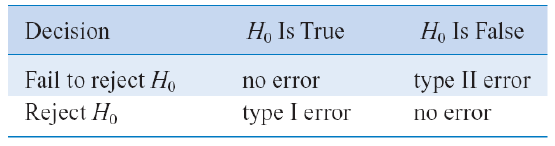
\includegraphics[scale=0.5]{testing}
\end{center}

\newpage

Idea follows US justice system.  Consider the following example:\\~\\
A person is on trial for a crime.	
\begin{itemize}
\item The null hypothesis is $H_0$: Innocent  
\item The alternative is $H_A$: Guilty
\begin{itemize}
\item A type I error would be \\
\item A type II error would be \\
\end{itemize}
\end{itemize}
For most crimes, a type I error is worse than a type II.  This is the same in an experiment, usually making a type I error is worse, so we set \textit{the type I error rate} at $\alpha$.\\~\\~\\

For the light bulb example earlier, what would a type I error be in words?  a type II error?\\~\\~\\~\\~\\~\\~\\~\\~\\

\large Step 3 - Check Assumptions and Find Test Statistic\normalsize\\~\\
To make inference, we will need a `test statistic' (such as $\bar{Y}$ or $Z=\frac{\bar{Y}-\mu_Y}{\sigma_Y/\sqrt{n}}$) that we know the \textit{sampling distribution} of.\\~\\

Recall:  If we are interested in a true mean, we can estimate it using the sample mean (a RV).  We know the distribution of the sample mean is 
$$\bar{Y}\sim N(\mu_Y,\sigma^2_Y/n)$$ 
if\\~\\~\\~\\~\\~\\~\\

We assume the null hypothesis is true and see if we find evidence to the contrary.\\~\\
Assuming the null hypothesis is true, we can use the test statistic

\newpage

For the two examples previously given, 
\begin{itemize}
\item determine which assumptions are met,
\item calculate the \textbf{observed} value of the test statistic,
\item assuming the null is true, draw the sampling distribution and place the observed value of the test statistic on the distribution.
\end{itemize}

\newpage

\large Step 4 - Find Rejection Region (RR) and/or find P-value - Make Decision\normalsize\\~\\
\underbar{~~~~~~~~~~~~~~~~~~~~~~~~~~~~~~~~~~~~~~~~~~~~~~~~} is determined by our chosen $\alpha$ and the distribution of our test statistic under the null hypothesis.\\~\\
RR - values of the test statistic for which the null hypothesis will be rejected.\\~\\
For a `$>$' alternative and an $\alpha=0.05$ let's find our RR\\~\\~\\~\\~\\~\\~\\

For a `$<$' alternative and an $\alpha=0.01$ let's find our RR\\~\\~\\~\\~\\~\\~\\

For a `$\neq$' alternative and an $\alpha=0.05$ let's find our RR\\~\\~\\~\\~\\~\\~\\

For the previous two examples, let's write down our RR and make our decision using $\alpha=0.05$.

\newpage

\underbar{~~~~~~~~~~~~~~~~~~~~~~~~~~~~~~~~~~~~~~~~~} - probability of getting a test statistic as extreme or more extreme than the observed value, assuming the null hypothesis is true.
\begin{itemize}
\item Measure of how likely it is to get this type of sample (or worse) if $H_0$ is true.
\item A better measure than RR for evaluating the evidence for or against the null. 
\end{itemize}
For a `$>$' alternative the p-value is\\~\\~\\~\\~\\
For a `$<$' alternative the p-value is\\~\\~\\~\\~\\
For a `$\neq$' alternative the p-value is\\~\\~\\~\\~\\
Decision determined by
\begin{itemize}
\item If p-value $\leq\alpha$, \underbar{~~~~~~~~~~~~~~~~~~~~~~~~~~~~~~~~~~~~~~~~~~~~~~~~~~~~~~~~~~~~~~~~~~}\\
\item If p-value $>\alpha$, \underbar{~~~~~~~~~~~~~~~~~~~~~~~~~~~~~~~~~~~~~~~~~~~~~~~~~~~~~~~~~~~~~~~~~~~~~}
\end{itemize}

For the previous two examples, let's draw the sampling distribution of the test statistic, shade the `extreme' region, find the p-value, and make our decision using $\alpha=0.05$.

\newpage

\large Step 5  - Draw Conclusions (in the context of the problem)\normalsize\\~\\

Interpreting the result means that we say in a formal way what our conclusion means for this problem:
\begin{itemize}
\item Fail to reject $H_0$, we say... At the $\alpha$100\% significance level, there is not enough evidence to support the alternative hypothesis that (context).
\item Reject $H_0$, we say... At the $\alpha$100\% significance level, there is enough evidence to reject the null hypothesis that (context) in favor of the alternative that (context).
\end{itemize}
For the previous two examples, let's interpret our results at the 0.05 significance level.  \\~\\~\\~\\~\\~\\~\\~\\~\\~\\~\\~\\~\\~\\~\\~\\~\\~\\~\\~\\~\\~\\~\\~\\~\\~\\~\\

Overview of HT
\begin{enumerate}
\item Set up Alternative
\item Set up Null
\item Check Assumptions and Calculate Observed Test Stat
\item Find RR and/or P-value
\item Draw Conclusions in the context of the problem
\end{enumerate}

\newpage

Example: The average employee tenure (number of years workers have been with their current employer) in 2010 was 4.4 years with a standard deviation of 0.9 years. Tenure is believed to be higher in this year than it was in 2010. A sample of 90 employees produced a mean tenure period of 4.7 years. 
\begin{enumerate}
\item Assuming the spread remained constant, conduct a 0.01 level (that means use $\alpha=0.01$) test to determine if average tenure is greater than it was in 2010. (You need to do all 5 steps.)
\item Is the sample mean 4.7 `significantly different' from 4.4?  Explain what we mean by significantly different in the context of the problem.
\end{enumerate}

\newpage


Relationship between CIs and Two-sided Tests
\begin{itemize}
\item If the null value $\mu_0$ is contained in a $100(1-\alpha)$\% CI for $\mu$, then we fail to reject $H_0$ at level $\alpha$.
\item If the null value $\mu_0$ is NOT contained in a $100(1-\alpha)$\% CI for $\mu$, then we reject $H_0$ at level $\alpha$.\\~\\~\\~\\~\\~\\~\\~\\~\\~\\
\end{itemize}

Let's calculate a confidence interval for $\mu$ in the employee tenure example.

\newpage

\Large 5.5 - Power and Choosing a Sample Size \normalsize\\~\\

\underbar{~~~~~~~~~~~~~~~~~~~~~~~~~~~~~~~~~} = 1 - P(Type II Error) = 1-$\beta$ = 1 - P(failing to reject $H_0$ when $H_A$ is true) = P(reject $H_0$ when $H_A$ is true)\\~\\

Ideally, we have small type I AND type II error rates (probabilities).  \\
We `control' the $\alpha$ = P(type I error) = type I error rate by setting this prior to the experiment.  \\
The main way to deal with the type II error rate (or equivalently power) is by increasing the sample size.\\~\\

Ex:  The drying time of a certain type of paint (in minutes) under specified test conditions is known to follow a $N(75,9^2)$. Chemists have designed a new additive to decrease average drying time. Let Y denote the drying time of this new additive. Let’s assume the $Y\sim N(\mu,9^2)$. We want to determine if there is strong evidence to suggest an improvement in average drying time. Suppose a random sample of 25 drying times is taken and the sample mean is 70.8.
\begin{enumerate}
\item Conduct a hypothesis test using rejecting regions and $\alpha = 0.01$.

\newpage

\item A HT is conducted assuming $H_0$ is true.  Let the random sample of 25 drying times be denoted as 𝑌$Y_1,𝑌Y_2,...,𝑌Y_{25}$. What is the distribution of $\bar{Y}$ generally? \\~\\~\\~\\~\\
\item Assume now that in actuality the average drying time is truly 72 minutes. Find the probability of a type II error. (We denote this as $\beta(72)$.) 
\begin{flushleft}
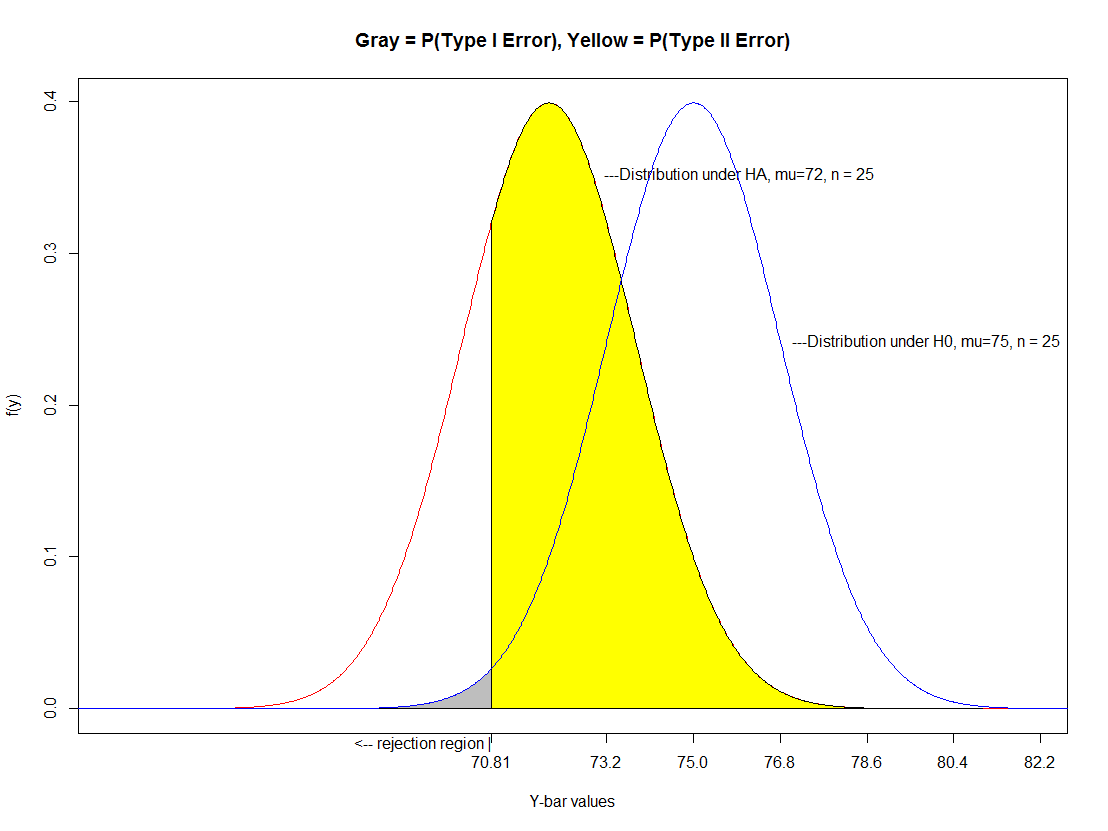
\includegraphics[scale=0.3]{mu72n25}
\end{flushleft}
\item Assume now that in actuality the average drying time is 70 minutes. Find the probability of a type II error, 𝛽$\beta(70)$.
\begin{flushleft}
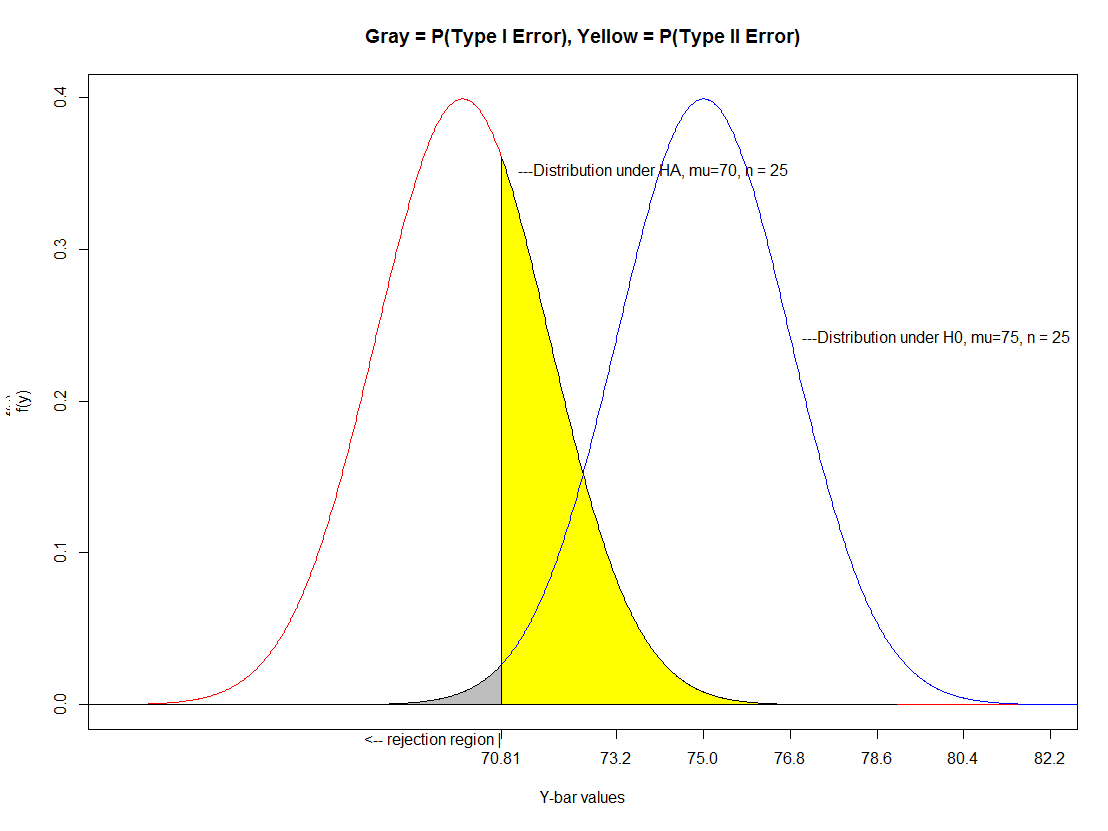
\includegraphics[scale=0.3]{mu70n25}
\end{flushleft}
~\\
\newpage

\item Continuing with the assumption that $\mu=70$, suppose now that a random sample of size n=49 is conducted.  Find $\beta(70)$.
\begin{flushleft}
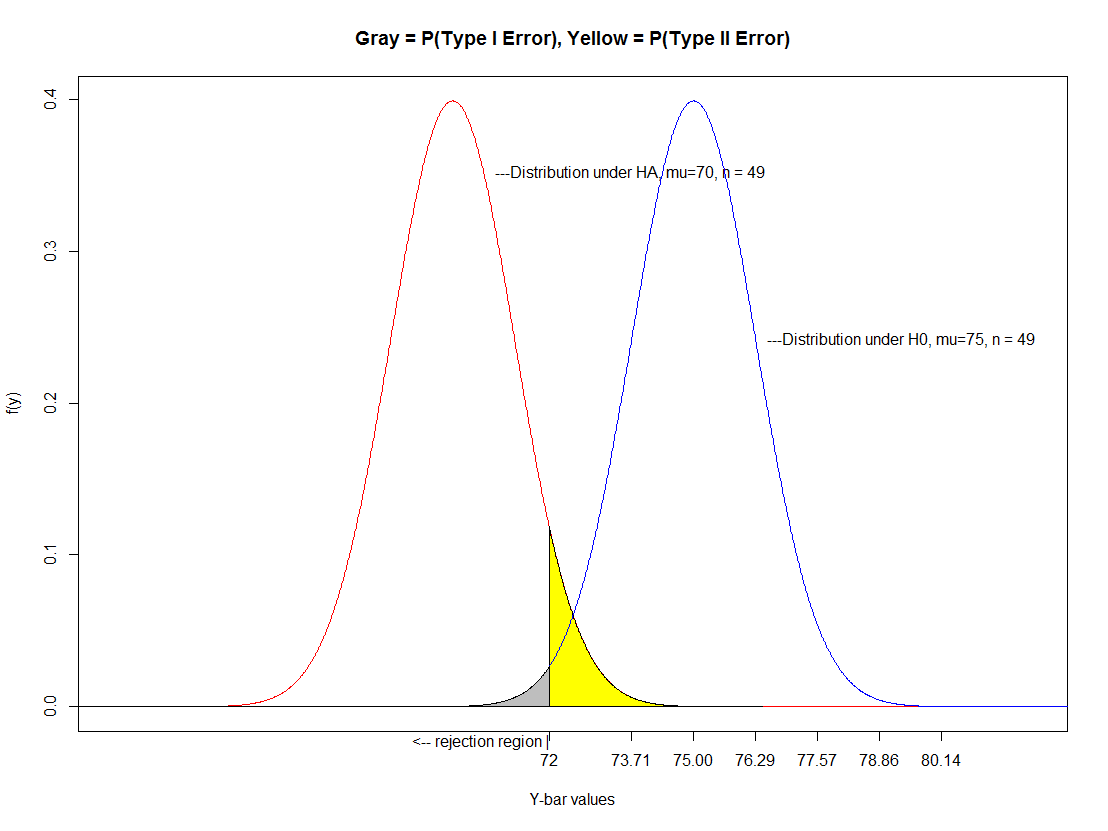
\includegraphics[scale=0.3]{mu70n49}
\end{flushleft}
\end{enumerate}

Generally, the type II error rate for a one-tailed test is given by
$$\beta(\mu_A)=P\left(Z\leq z_\alpha - \frac{|\mu_0-\mu_A|}{\sigma/\sqrt{n}}\right)$$
for a two-tailed test it is given by
$$\beta(\mu_A)\approx P\left(Z\leq z_{\alpha/2} - \frac{|\mu_0-\mu_A|}{\sigma/\sqrt{n}}\right)$$
Prior to an experiment, we would assume a value for $\sigma_Y$ and plot the power (or type II error rate, $\beta$) as a function of $\mu_A$.  
\begin{flushleft}
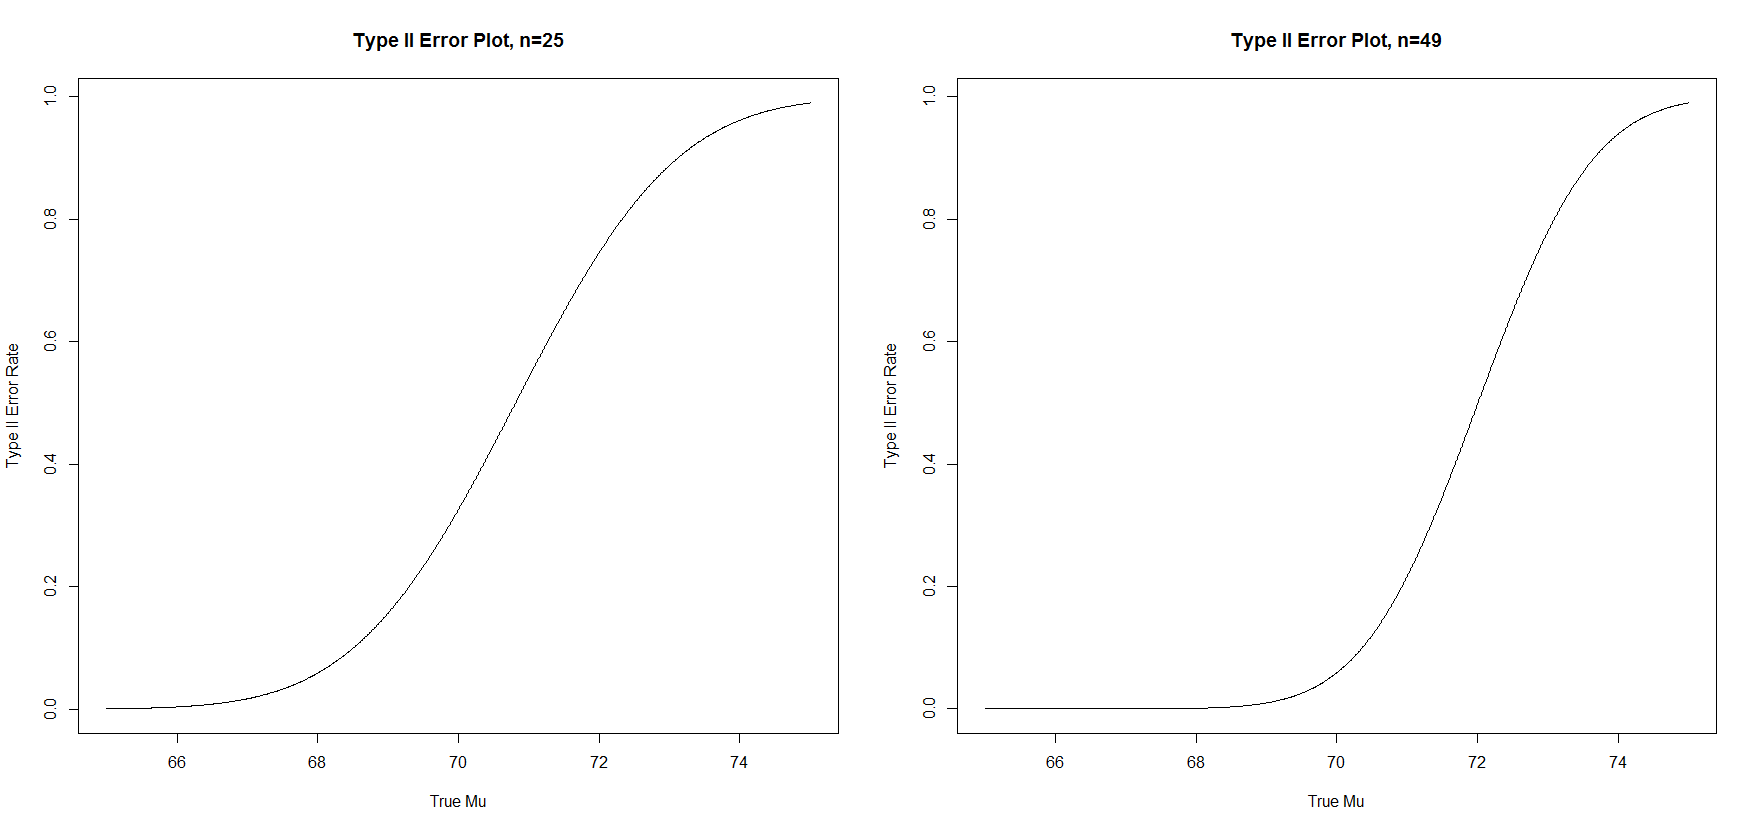
\includegraphics[scale=0.3]{typeIIerrorplot}
\end{flushleft}
\begin{flushleft}
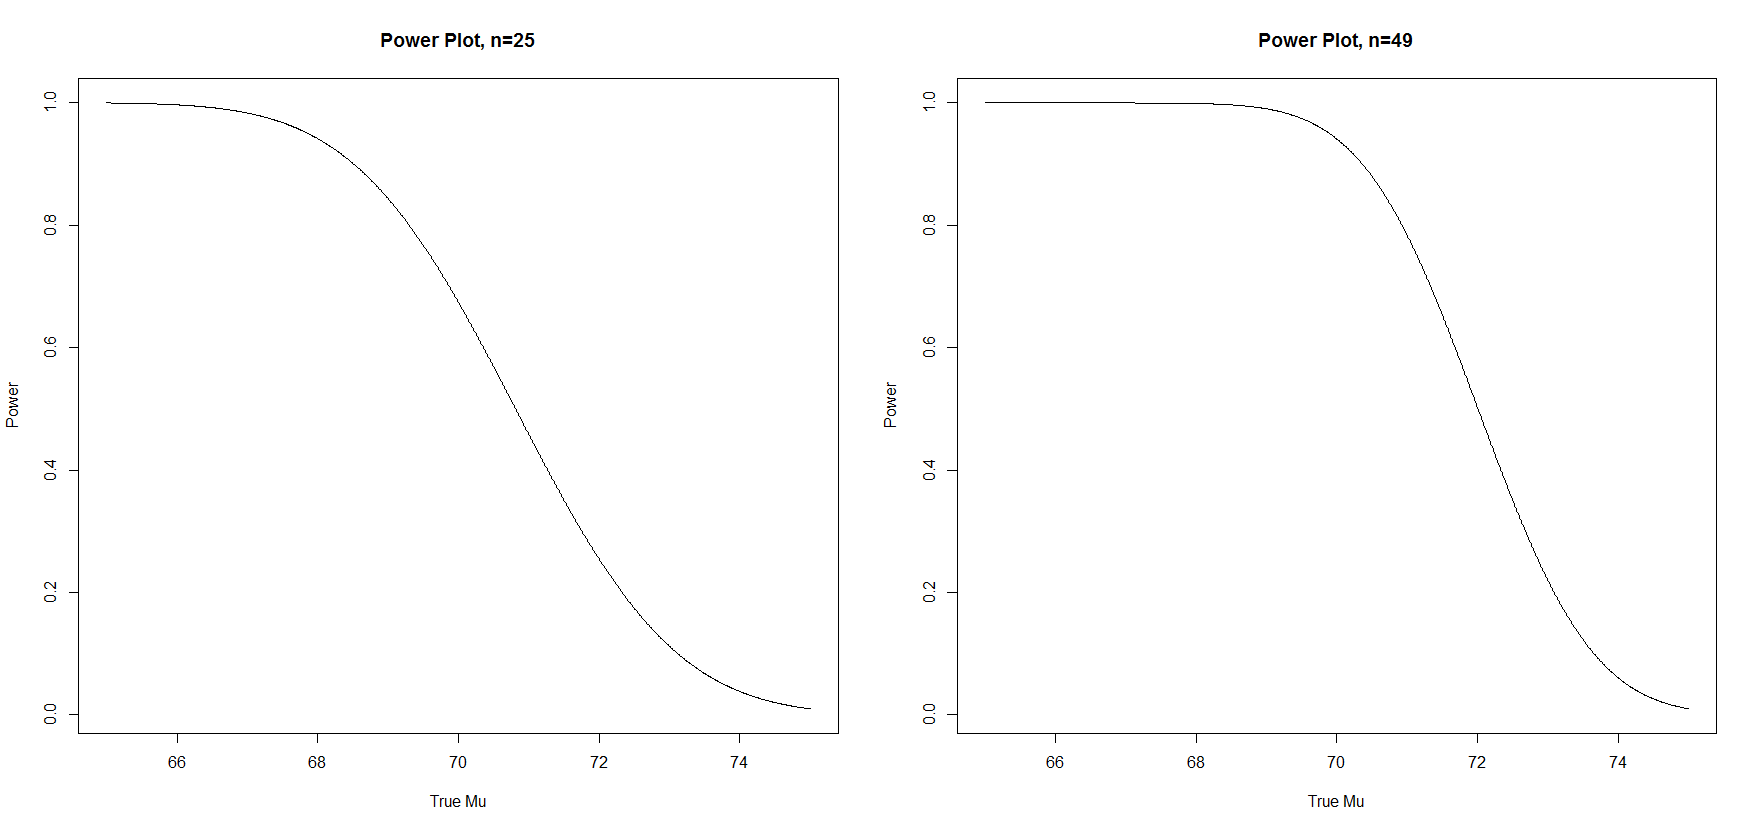
\includegraphics[scale=0.3]{powerplot}
\end{flushleft}

Recall Example: The average age of a person on facebook last year was 19.34 years.  The standard deviation of the age of facebook users is 8.2 years.  Suppose an advertising agency is interested in seeing if the average age is different this year. He randomly selects 150 profiles and finds that the sample mean is 18.99 years old.\\~\\
Using $\alpha=0.05$, our RR is $\left\{z_{obs}:|z_{obs}|>1.96\right\}$.\\~\\
What is the power if $\mu_A=18$ is the truth?  if $\mu_A=21$ is the truth?\\~\\~\\~\\~\\~\\~\\~\\~\\~\\
Looking at the power curve below, what is the power when $\mu=19.34$ is the truth?  Why does this make sense?\\~\\
\begin{flushleft}
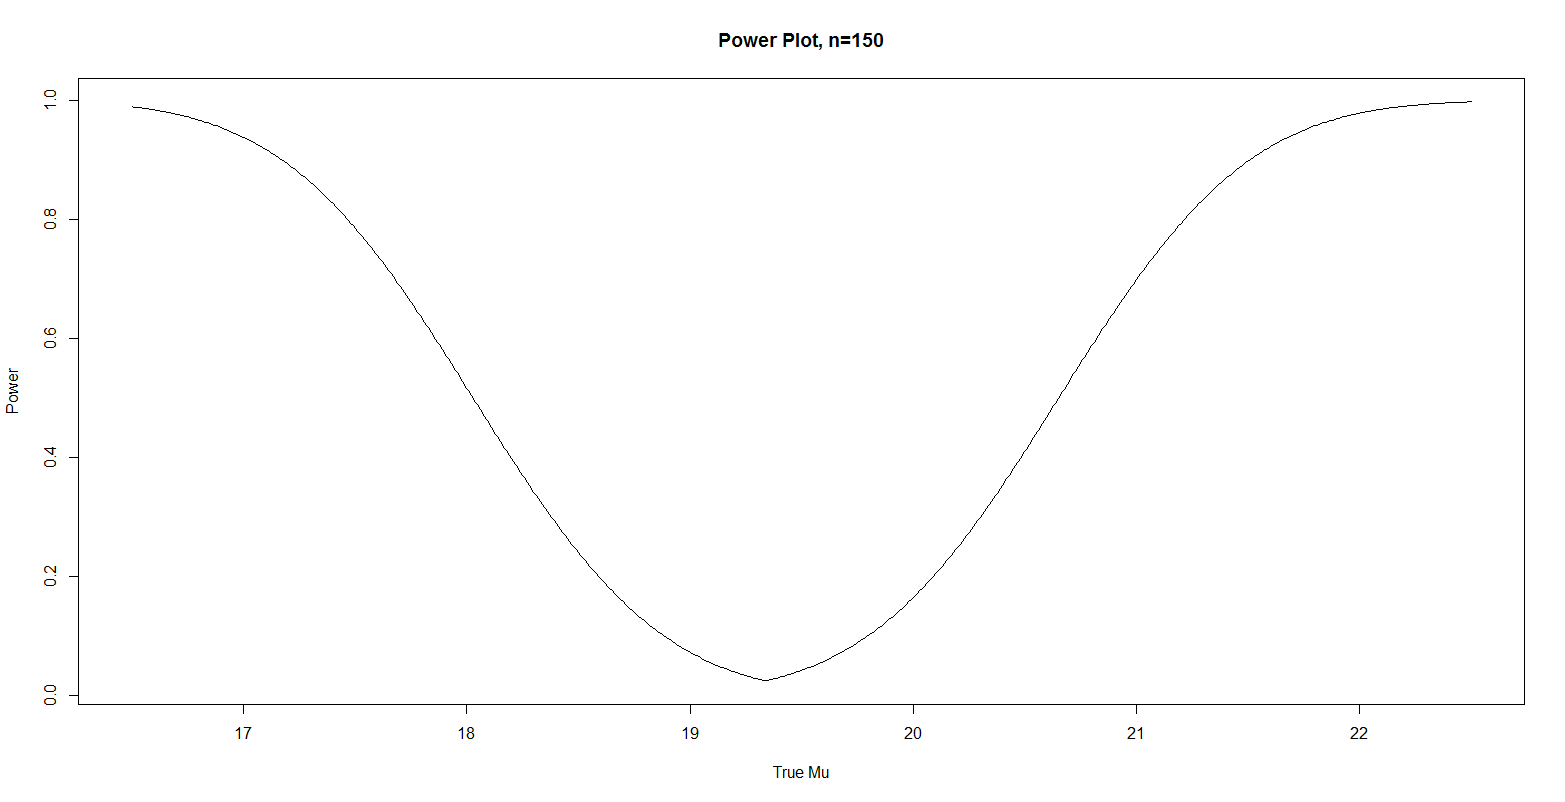
\includegraphics[scale=0.2]{powerplot2}
\end{flushleft}

\newpage

Alternatively, we could fix the value of $\mu_A$ and let n vary to determine a given sample size for obtaining a certain power.\\~\\
Drying time example with $\mu_A=72$.  Plot of power for varying n
\begin{flushleft}
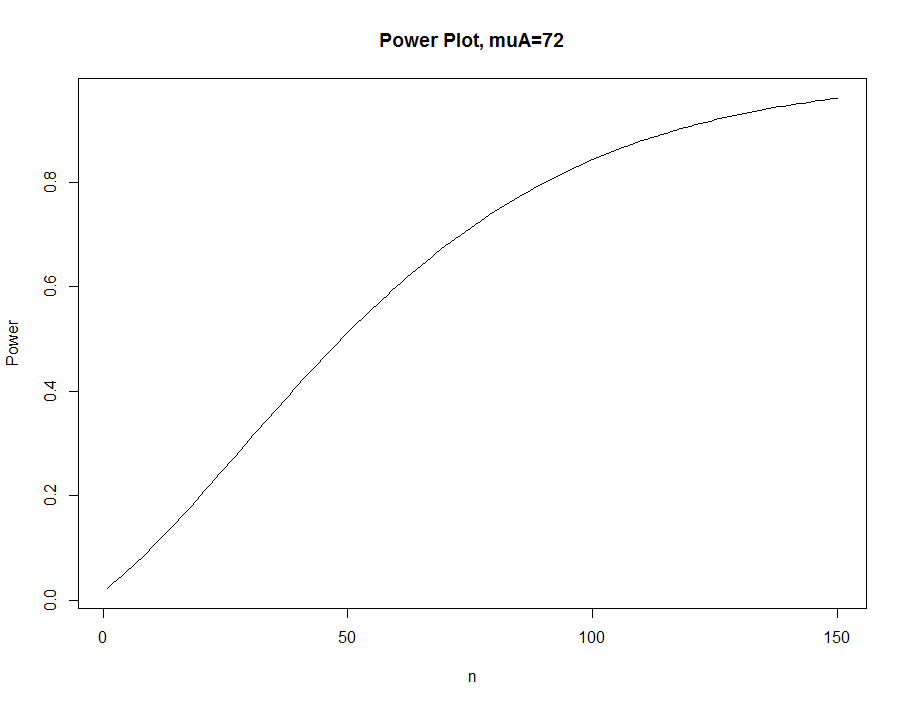
\includegraphics[scale=0.3]{powerplot3}
\end{flushleft}
~\\~\\
Facebook age example with $\mu_A=18$.  Plot of power for varying n
\begin{flushleft}
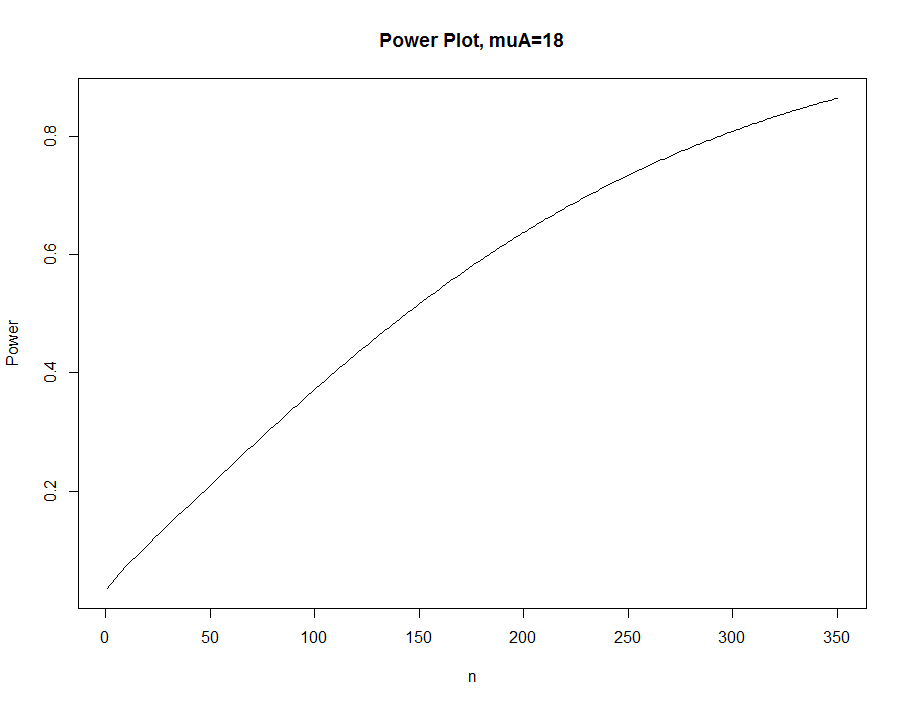
\includegraphics[scale=0.3]{powerplot4}
\end{flushleft}




